% \documentclass[fleqn,10pt]{wlscirep}
% \usepackage[utf8]{inputenc}
% \usepackage[T1]{fontenc}
% \usepackage{float}
% \usepackage{xcolor}
% \usepackage{enumitem,amssymb}
% \usepackage{subcaption}
% \newlist{checklist}{itemize}{2}
% \setlist[checklist]{label=$\square$}
% \usepackage{longtable}
% \usepackage{soul}
% \usepackage{longtable}
% \newcommand{\notateThiago}[1]{\textcolor{blue}{\textbf{[#1]}}}
% \newcommand{\notateJay}[1]{\textcolor{red}{\textbf{[#1]}}}
% \newcommand{\doiprefix}{}
% \counterwithin{figure}{section}


% \title{In-flight positional and energy use data set of a DJI
% Matrice 100 quadcopter for small package delivery
% : Supplementary information}
% \begin{document}
% \author{}
% \maketitle

\section{Checklists}
\subsection{Pre-Flight}
\label{apen1:pre}

\begin{checklist}
    \item Inspect the aircraft 
    \begin{checklist}
        \item Visually inspect the condition of the unmanned aircraft system components
        \item Inspect the airframe structure, including undercarriage, all flight control surfaces and linkages
        \item Inspect registration markings for proper display and legibility
        \item Inspect moveable control surface(s), including airframe attachment point(s)
        \item Inspect servo motor(s), including attachment point(s)
        \item Inspect the propulsion system, including powerplant(s), propeller(s), rotor(s), ducted fan(s), etc.
    \end{checklist}
    \item Verify all systems (e.g. aircraft, control unit) have an adequate energy supply for the intended operation and are functioning properly
    \item Inspect the avionics, including control link transceiver, communication/navigation equipment and antenna(s)
    \item Check UAS compass and calibrate UAS compass prior to any flight if necessary.
    % \item Inspect the control link transceiver, communication/navigation data link transceiver, and antenna(s)
    \item Check that the display panel, if used, is functioning properly
    \item Check ground support equipment, including takeoff and landing systems, for proper operation
    % \item Check that control link correct functionality is established between the aircraft and the control station
    % \item Check for correct movement of control surfaces using the control station
    \item Check on board navigation and communication data links
    \item Check flight termination system and manual override switch
    % \item Check fuel for correct type and quantity
    \item Check battery levels for the aircraft and control station
    \item Check that the payload is securely attached
    \item Verify communication with UAS and that the UAS has acquired GPS location from at least 4 satellites
    \item Arm and disarm the UAS propellers to inspect for any imbalance or irregular operation
    % \item Verify all controller operation for heading and altitude
    \item If required by flight path walk through, verify any noted obstructions that may interfere with the UAS
    \item At a controlled low altitude, fly manually within range of any interference and recheck all controls and stability
\end{checklist}

\subsection{Post-Flight}
\label{apen1:post}
% \subsection*{Pre-landing}
% \begin{checklist}
%     \item Ensure that the LZ (landing zone) is clear, otherwise abort and proceed to alternative LZ
%     \item Pilot calls "Landing"
%     \item Initiate auto land either using the app or programming code
% \end{checklist}

% \subsection*{Post-landing}
\begin{checklist}
    \item Wait for all motors and rotors to stop
    \item Verify stop sensor recording
    \item Disconnect the battery
    \item Inspect the airframe for any in-flight damage
    \item Check wiring is secure
    \item Check connectors are fully connected
    \item Motors are securely mounted
    \item Propellers are securely fastened
    \item Propellers rotate freely without any obstructions (e.g. hitting edges of incorrectly fitted indoor hull) or have been removed.
    \item All sensors are unobstructed and undamaged
\end{checklist}

\section{Anemometer Magnitude Bias and Ego Motion Correction}
\label{chap:bias}

One way to remove the magnitude bias and ego motion in the wind measurements is by using the inertial velocity data and the data collected by Brushi et al. \cite{bruschi2016wind} of a quadrotor flying with a ultrasonic wind sensor inside a wind tunnel. Given the similarity between our setup and theirs, the wind-tunnel results\cite{bruschi2016wind} are used to construct a polynomial mapping between measured and actual wind speeds. As the data lacks points in the lower range of values, it is augmented with results from our own setup. The data-points and the curve fit are plotted in Figure \ref{fig:anemo_usage}. The UAV was flown in hover and constant ground speed mode for an extended amount of time in near-zero wind conditions to get the lower range of values. The magnitude correction polynomial and ego-motion correction is given in Equation \ref{eq:corr}.
\begin{equation}
    \begin{split}
% V &= \sqrt{V_N^2 + V_E^2}\\
w_m^{[actual]} &= -0.002(w_m^{[raw]})^4 + 0.052(w_m^{[raw]})^3-0.421(w_m^{[raw]})^2 + 1.917w_m^{[raw]} - 2.7\\
w_N &= (w_m^{[actual]})\cos(w_{\theta}^{[raw]}) - V_N\\
w_E &= (w_m^{[actual]})\sin(w_{\theta}^{[raw]}) - V_E\\
w_m^{[corrected]} &= \sqrt{w_N^2 + w_E^2}\\
w_{\theta}^{[corrected]} &= \arctan(w_E,w_N)\\
\end{split}
\label{eq:corr}
\end{equation}
where $V_N$ and $V_E$ represent the inertial speed of the UAV in North and East directions, and $w_N$ and $w_E$ represent the corrected wind components in North and East directions. 
\begin{figure} [H]
    \centering
    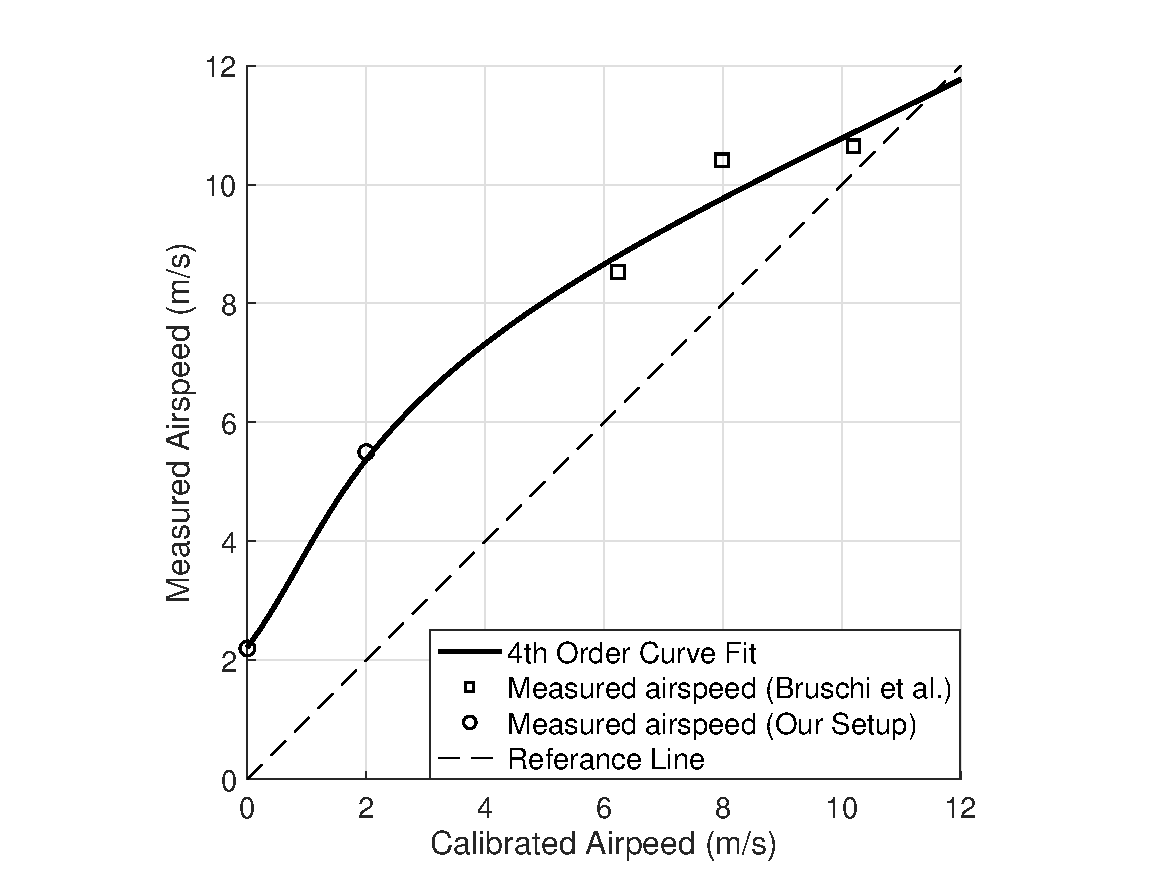
\includegraphics[width=0.45\textwidth]{figures/figure11.pdf}
    \caption{Anemometer corrections}
    \label{fig:anemo_usage}
\end{figure}

The data set contains the raw measurements and is not modified with these proposed methods, as the focus of this work is not about obtaining accurate wind field estimations. The area of wind estimation through the use of a drone is an ongoing field of research\cite{Patrikar-2020-125335}, as the rotors induce complex air disturbances which affect the anemometer. Thus we left our data in a state where various current or future methods of wind correction can be applied if needed.

% \end{document}